\section{Multitouch Table}
You will be assimilated (see figure \ref{fig:mtdiagram}). 
\begin{figure}[htp]\centering
  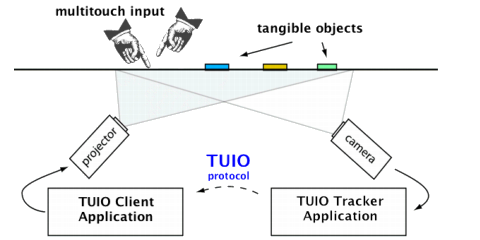
\includegraphics[width=.8\textwidth]{images/mt-diagram.png}
  \caption{This is a multitouch table!}\label{fig:mtdiagram}
\end{figure}
\subsection{Software}
The multitouch table uses The Beta, from the NUI Group \cite{NUI}, to process the video stream from the webcam. The Beta, tbeta for short, is an open source tool that analyzes a video to find tracking data for objects it recognizes as fingers or cursor devices. The software provides a great deal of control over the video parameters (high-pass filter, amplification, threshold, etc.) that adapts well to many types of multitouch displays.

Tbeta outputs the tracking data using the TUIO protocol \cite{TUIO}, which is an open framework for receiving input events in various programming environments. For this project, the TUIO events sent by tbeta were received using the open source Java TUIO library in a Processing sketch. 
